% easychair.tex,v 3.5 2017/03/15

%\documentclass{easychair}
\documentclass[EPiC]{easychair} % this is for ISCA conference proceedings
%\documentclass[EPiCempty]{easychair}
%\documentclass[debug]{easychair}
%\documentclass[verbose]{easychair}
%\documentclass[notimes]{easychair}
%\documentclass[withtimes]{easychair}
%\documentclass[a4paper]{easychair}
%\documentclass[letterpaper]{easychair}

\usepackage{doc}

% use this if you have a long article and want to create an index
% \usepackage{makeidx}
% In order to save space or manage large tables or figures in a
% landcape-like text, you can use the rotating and pdflscape
% packages. Uncomment the desired from the below.
%
% \usepackage{rotating}
% \usepackage{pdflscape}
% Some of our commands for this guide.
%
\newcommand{\easychair}{\textsf{easychair}}
\newcommand{\miktex}{MiK{\TeX}}
\newcommand{\texniccenter}{{\TeX}nicCenter}
\newcommand{\makefile}{\texttt{Makefile}}
\newcommand{\latexeditor}{LEd}

%\pagestyle{empty}
%\makeindex
%% Front Matter
%%
% Regular title as in the article class.
%
\title{Re-engineering legacy enterprise content management (ECM) systems for cloud-environments
%    \thanks{With contributions from Gang,Shao via his master thesis at the University of Stuttgart.}
    }

% Authors are joined by \and. Their affiliations are given by \inst, which indexes
% into the list defined using \institute
%
\author{ Cataldo Mega\inst{1}
%\thanks{Designed and implemented the legacy and cloud version of the ECM prototype}
 % \and
%	Gang Shao \inst{1}\thanks{Implemented the docker version of the ECM prototype}
}


% Institutes for affiliations are also joined by \and,
\institute{ 
	University of Stuttgart, Stuttgart, IPVS, Germany\\
	\email{cataldo.mega@ipvs.uni-stuttgart.de}
}

%  \authorrunning{} has to be set for the shorter version of the authors' names;
% otherwise a warning will be rendered in the running heads. When processed by
% EasyChair, this command is mandatory: a document without \authorrunning
% will be rejected by EasyChair

\authorrunning{C.,Mega}

% \titlerunning{} has to be set to either the main title or its shorter
% version for the running heads. When processed by
% EasyChair, this command is mandatory: a document without \titlerunning
% will be rejected by EasyChair
\titlerunning{Re-engineering legacy ECM systems for cloud-environments}

\begin{document}

\maketitle

\begin{abstract}
  %Enterprise content management (ECM) systems are the custodians of unstructured enterprise data,  As such, 
  %ECM systems are the common unstructured data repository and enterprise archive in support of the corporate information life cycle and governance strategy as well as implementing records management and legal e-discovery. Over the last decades, legacy ECM production environments and related application development, test and provisioning processes have become slow, inflexible and too expensive in order for being competitive with cloud native solutions. However, 
  Considering the cloud promises, our investigations aim at answering the following questions: i) can we boost productivity and still reduce administrative and operations costs?, ii) can long-term IT-capital investment costs (CAPEX) be transformed in short-term operational expenses (OPEX)? and finally iii) is it possible to grow business with the same IT-personnel? The results of our investigations and analysis indicate that there are positive answers to those questions.
  Our investigations show that by properly re-engineering legacy ECM systems existing design shortcomings can be removed and gaps closed by evolving the architecture from an old client-server-computing into a modern cloud-computing model. To prove our claims we implemented both, a legacy ECM system using it as a reference and a virtualized/containerized ECM systems running on a OpenStack-KVM-Docker cloud platform. Then we compared the cloud against the classical approach. The focus of our analysis was to understand the different operational aspects required for setting up the legacy and cloud IT run-time environments and the changes required to re-engineer the system component configuration and resulting deployment topology. We found that some of the design pattern implementations used in the client-server-computing model are no longer adequate in the cloud-computing world, thus preventing the exploitation of new features of the cloud platform such as dynamic deployment, load balancing and elasticity. First results show that by applying the right corrective measures it is possible to ready legacy ECM systems for the Cloud.\footnote{we use the term 'the Cloud' as a synonym for 'cloud environments'}
 % and successfully run them in kubernetes/docker based cloud environments.
 \end{abstract}
 
  \paragraph{Keywords.} Enterprise content management, architecture design, cloud-computing model.

% The table of contents below is added for your convenience. Please do not use
% the table of contents if you are preparing your paper for publication in the
% EPiC Series or Kalpa Publications series
%\setcounter{tocdepth}{2}
%{\small
%\tableofcontents}
%\section{To mention}
%
%Processing in EasyChair - number of pages.
%
%Examples of how EasyChair processes papers. Caveats (replacement of EC
%class, errors).
%-------------------------------------------------------------
\section{Short... Introduction ... ECM and cloud}
\label{sect:introduction}
  (Mehr quellen ... die belegen was ich sage)
  Cloud computing \cite{FehlingLRS2011} has become synonymous with a faster, scalable, flexible and cost-efficient IT infrastructure offered as an online service. Intrigued by these promises, chief officers (CxO) in companies are driving the restructuring of their ECM IT environment as the legacy provisioning processes have become slow, inflexible and too expensive. These circumstances led to an erosion of competitiveness against cloud native solutions.\textit{(proof it ... eg box, drop box, amazon,compliance repository )} On the other hand, what has been working well for years and where substantial investments have been made cannot be thrown over-board just like this. Therefore, it is worth the challenge to create a content management as a service (CMaaS) offering tailored for the B2B Eco-system, in which to build quickly an attractive and profitable food chain with cloud-enabled ECM systems. In order to develop possible solution strategies, it is necessary to understand what the actual technical impediments are and answering the following questions: i) is it possible to evolve the old legacy ECM systems design and ready it for the ‘Cloud’ or ii) is it better to slowly phase it out and replace existing legacy with cloud native versions. To achieve these goals, we investigated the architecture design changes required for the cloud and analyzed their workload pattern. Our approach was to determine the shortcomings of the outdated client-server computing model employed and compare it against the cloud-computing model in wide adoption today.
  % ... workload related to document management, compliance archiving, records management and e-discovery
  With this first work, we develop a virtualized and containerized ECM prototype by decomposing the application stack into components that are confined in stand-alone docker containers, deployed in a virtualized IT environment that is set up through an automated roll-out process. Our investigation surfaced several design hot spots and we found ways to evolve the legacy client-server architecture design into a cloud-computing one. The lessons learned show that it is possible to re-engineer an ECM system such to exploit cloud technology and to successfully compete against cloud native competitors. 
  
  The remainder of this paper is structured as follows: In Section 2, we describe the foundations of ECM and define the context in which this work is embedded. Section 3 highlights some of the more important areas of related work that further expands the ECM context and where we found motivation for our investigations. Section 4 lists the relevant business and functional requirements which we used as guidelines for de-composing the ECM application into consumable function units. Section 5 introduces the logical deployment model and Section 6 the derived implementation model of our prototype. Section 7 is dedicated to our analysis and the results of our investigation. Section 8 presents our conclusions and provides an outlook of ongoing current and planned future software re-engineering work in this field. 

  \noindent \paragraph{\textbf{Our goals}} Now, considering the cloud promises, our investigations aim at answering the following questions: i) can we boost productivity and still reduce administrative and operations costs?, ii) can long-term IT-capital investment costs (CAPEX) be transformed in short-term operational expenses (OPEX)? and finally iii) is it possible to grow business with the same IT-personnel? The results of our investigations and analysis indicate that there are positive answers to those questions.
    
%------------------------------------------------------------------------------------------------
\section{Foundation and related work}
\label{sect:foundation}
%\subsection{Definition of enterprise content management }
    The Association for Information and Image Management (AIIM) defines Enterprise Content Management as follows~\cite{AIIM-2020}: \textit{"Enterprise Content Management is the systematic collection and organization of information through a combination of strategies, methods, and tools used to capture, manage, store, preserve, and deliver information in support of the enterprise life cycle and governance processes.”}  \noindent In this paper, the term \textit{information} refers to \textit{content} any kind and any type of unstructured business data, be it in form of office-documents, files, images, audio, video or any other multi-media content. \textit{Meta-data} is the companion term and refers to information about the \textit{content} and its relation to the business it belongs to. More specifically, \textit{meta-data} relates also to management and operational information required to support the corporate information life cycle, governance and compliance processes. Thus technically speaking ECM can be thought of as being the governance practice that handles the information life cycle in a heterogeneous, geographically distributed corporate unstructured data landscape.\textbf{Reimer, James.A.}\cite{reimer-james} in his paper outlines the basics of ECM system its structure, function, and the extensions and adds a discussion on the type of workloads that typical unstructured data services generates. \textbf{Brocke vom,Jan} \cite{vom-Brocke} further elaborates on the functional aspects of ECM and presents an ECM-blueprinting framework. Shiva Hullavarad  \cite{Shiva-Hullavarad} in his paper explained the benefit of moving ECM in to the cloud and predicted this trend would gain momentum.
    
    %and ultimately the actual motivation behind the existence of ECM Systems. Thus, ECM answers the following fundamental enterprise governance questions: i) What kind and type of data exists and where is the data coming from? ii) Is the data properly classified, secured. iii) who is the responsible custodian ?, iv) who needs or is authorized to access the data, and v) for how long must it be retained before it is defensible disposed? \textit{Governance}, among many other aspects, implies that for every piece of relevant business data there must always exist an audit record such to withstand internal and external audits. The totality of these records represents the foundation of the \textit{enterprise content catalog}. The clear benefit of ECM is that by moving relevant content into an enterprise repository, this information becomes managed, controlled and stored in a compliant way.
    

%-----------------------------------------------------------
%\subsection{Related Work}
%\label{subsect:relatedwork}
     
    \textbf{Fehling et al.}~\cite{CloudComputingPatterns2014} in his \textit{Cloud Computing Patterns} book lists the fundamental cloud computing characteristics as being \textit{access via network, on-demand self-service, measured service (pay-per-use), resource pooling and rapid elasticity}. He explains that the latter \textbf{fundamentally change} how IT resources are provided and used. In conclusion, according to Fehling, the decision for the adoption of cloud offerings is based on typical application workload patterns. His findings guided our efforts to investigate how these properties are delivered on the different levels of a typical ECM application stack and under which conditions an ECM system will benefits from them. With the experience gained in the past decade we grow convinced that ECM successfully can cope with the new challenging trends and that with an appropriate re-design and a few enhancements to better exploit cloud technology it is possible to evolve ECM systems to successfully run in today's cloud environments. 
%---------------------------------------------------------------------------------------------------------------------------------------------
\section{ECM systems architecture design and blueprint}
\label{sect:architecture-design}
\subsection{Business and corporate requirements for ECM}
\label{subsect:business-requirements}
    In order to avoid confusions, in the context of this paper, we use the following terms interchangeably - "enterprise content information catalog", "central catalog", "master catalog" or simply "content catalog". It always implies a database schema holding all metadata relative to the managed content stored in the distributed physical content repositories.\\
    
    \noindent In companies, production environments store their unstructured business data and collateral materials on  back-office systems, file servers, email archives and other specialized storage locations. To ECM systems, these data silos represent the actual data sources from where, through specific integration points, relevant information is collected as mandated by business and corporate governance policies. For example, in the case of an insurance policy, after a lengthy chain of approval steps once the contract is signed it becomes immutable and the original copy needs to be stored away and securely managed through its life cycle based as mandated by corporate and legal policies. Overall information assets found are pre-classified into "business relevant" or "disposable after use". In the first case, the information is captured and loaded into the enterprise content repository for subsequent use. Thus, the business applications, corporate life-cycle and governance need at the core of an ECM system needs a capable content repository supporting and exposing the following characteristics:
\begin{itemize}
    \item BR-01 Collect, ingest and store business relevant information any type and format.
    \item BR-02 Classify, categorize and properly tag information relevant to business and corporate compliance.
    \item BR-03 Provide a flexible metadata management and an efficient information retrieval service in support of an enterprise wide document management and archiving offering.
\end{itemize}

\subsection{ Functional and non-functional requirements } 
\label{sect:functional-requirements}

    Usually the collection, classification and the ingest of information is done by components running outside of the core ECM system and will did consider them in this work. Instead, we focused more on business requirement BR-03 which we translate into the following functional and non functional requirements.\\
    \noindent \textbf{Functional requirements -} As we said before, the expectation for ECM systems is that they efficiently handle the ingest of unstructured data loaded at variable rates by a possibly large population of end users and applications. Upon loaded, there is a chain of sub-processes that the content is pushed through, ranging from indexing, to transformation, encryption and de-duplication before the content in the end is persisted on designated geographically distributed storage systems.These BR-01-B02 related services will develop an \textit{I/O intensive variable workload}. In the opposite direction as part of BR03, the retrieval process is based on a flexible information retrieval system supporting different retrieval technologies including relational, free-text, and more recently ML and AI technologies. Thus the BR-03 services do generate a more \textit{CPU intensive variable workload}. The functional scope that can be derived from BR01-BR03 includes: \\- FR-01) - a pre-defined repository data model, \\FR-02) - integration points that allow business applications specific entities metadata-extensions, \\- FR-03 - Keep strict referential integrity between meta-data and data avoiding dangling pointers and orphan objects,\\- FR-04) - information retrieval of unstructured data of any format and type, and \\- FR-05) - a flexible administration and management framework for implementing a corporate content life-cycle governance and disposal services. \\ The \textbf{non-functional requirements} for ECM systems can be summarized as follows: a) NFR-02 - gracefully cope with load variations by minimizing system disruptions such to ensure high availability and resilience to outages, and b) NFR-03 - Dynamically adapt the production-environment to current load variations by properly handling the commissioning and decommissioning of IT resources.
%-------------------------------------------------------------
    \noindent  \paragraph{ECM}reference architectures have been suggested by several sources\cite{reimer-james}, \cite{ECM-RA}, \cite{vom-Brocke}, \cite{Shiva-Hullavarad} which guided the design of our stripped down version of a ECM system architecture outlined in Figure~\ref{fig:architecture-blueprint}. It suggests five system layers and lists their respective components and services. There is the presentation layer, 2) business services layer, 3) content services layer, 4) resource services layer and the lowest 5) storage services layer. \\ \\
    \noindent  \textit{Layer-01 the presentation layer} can be thought as the "portal" to the corporate document repository and information archive. Second below is \textit{layer-02 the business layer} with content specific services addressing - capture, collection, ingest and delivery services residing outside of the core system. \textit{Layer-3 the content layer} encapsulates the core content services as being - central master catalog, modeling services, distributed transaction management, information retrieval, repository administration and governance execution services. \textit{Layer-04 the resource layer} is responsible for managing physical content and related storage sub-systems.This so called resource  manager uses a local object catalog to store, retrieve and deliver content in a transactional fashion. It also offers content transformation services like the de-duplication, encryption and rendition of content objects. Storage management services abstract from from distributed storage devices. \textit{Layer-05 the storage layer} consists of the logic to manage the different types content stores and to ensure  proper handling of the specialized storage access layer. \\
    
\begin{figure}[hbt!]
	\begin{centering}
	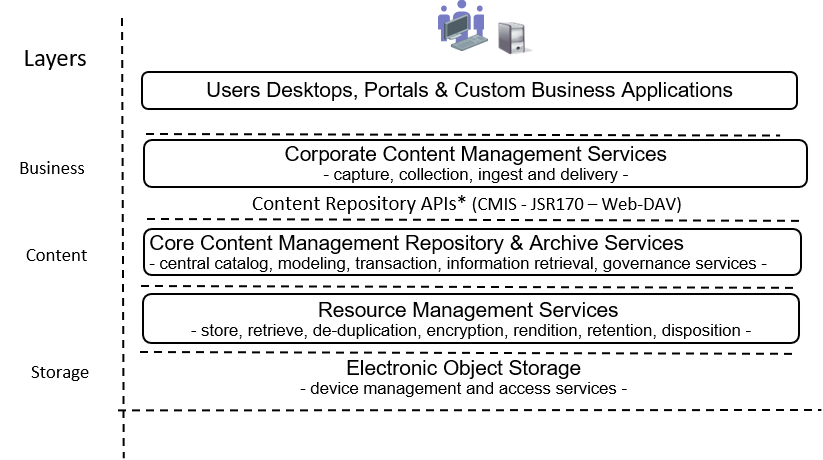
\includegraphics[width=0.75\textwidth]{pics/ECMPic04c.png}
	\caption{ECM architecture blueprint showing components by layer}
	\label{fig:architecture-blueprint}
	\end{centering}
\end{figure}

    \noindent We chose to have a deeper look at the content, resource, and storage layer as this is where we had identified the major hot-spots in need of the required cloud design re-engineering work. Our design analysis and layer-based decomposition effort focused therefore on the lower layers only. In the end we added also the ECM Portal component in order for us to build a complete end to end application stack.
    The end result was a set of components that would run and scale out independently in cloud environments consisting of: - content repository APIs, central catalog, object catalog, resource management services and content transformation services. From the outside world, access to all services exposed is through the published vendor specific ECM APIs. If cross-vendor ECM system access is required then the alternative is to use standard ECM APIs Content repository API for Java like \href{https://en.wikipedia.org/wiki/Content_repository_API_for_Java}{JSR-170}, Content Management Interoperability Services \href{https://en.wikipedia.org/wiki/Content_Management_Interoperability_Services}{CMIS} or even \href{https://en.wikipedia.org/wiki/WebDAV}{Web-DAV} in front of the proprietary API.
    %
    
% -----------------------------------------------------------------------------------------------
\section{ECM system logical deployment model}
\label{sect:ecm-deployment-model}
    % elaborate on this .......
    From an engineering stand-point the ECM repository concept relies on the \textit{"separation of concerns"} software design principle and employing a master/worker model. The master functions as the control center at the logical level. It uses the master data catalog for storing meta-data and coordinating all distributed transactions. Then, there are one or more dependent workers acting as a decentralized shared content repository. In practice, this means that meta-data management is separate from physical content management and, thus, the administration of the many physical content repositories are kept independent from the central meta-data catalog. By doing so and due to the employed \textit{location transparency}, stored electronic objects can be physically moved from one storage device to another or from one location to another based on business needs and compliance policies. Detail \textbf{D2} in Figure:~\ref{fig:ecm-model-deployment} below shows the distributed nature and linkage between the master and object catalogs, where data access to block-, file- and object-storage devices is provided by a dedicated data access component. The picture also states that transaction among the different components have to ensure strict consistency.    
    

\begin{figure}[hbt!]
	\begin{centering}
%	
\includegraphics[width=0.5\textwidth]{logoEC}
	\includegraphics[width=1.0\textwidth]{pics/ECMpic16a}
	\caption{ECM system logical deployment model}
	\label{fig:ecm-model-deployment}
	\end{centering}
\end{figure}
    
    \noindent From an implementation stand-point, the client-server computing way to deploy a distributed application was to design a multi-tier application system consisting of a HTTP server front-end connected to one or more Java Web Application Servers running Java2EE application components. The latter would talk to one or more databases. The preferred communication protocols were Web-Services, RPC and JDBC over https. At the very high level the deployment topology and its constituents look very much the same in both cloud and legacy environment. What changes is the  granularity of the service components and the refactored ECM application logic where in the past due to the lack of proper infrastructure support business logic was mangled with operational logic. Today hat is no longer necessary, cloud services can now handle all operational functions, application would declare what they need and the cloud IT-processes would deliver it.  

    \noindent Let us dive into the logical design by explaining how the individual ECM application components were packaged and and linked together in the deployment topology shown in Figure~\ref{fig:ecm-model-deployment}. We have defined application nodes of type \textit{N1-N5} and storage nodes \textit{SN1-SN2}. D1 and D2 are exploded details of the logical design used to explain other characteristics like: distributed transactional consistency, scale and availability. 
    
    %\noindent Leaving out the\textit{site load balancer}, represented by the scale icon and labeled \textbf{LB1} on the top left of    Figure~\ref{fig:ecm-model-deployment} 
    The left hand side diagram in Figure~\ref{fig:ecm-model-deployment} outlines the logical deployment model showing the minimum number of nodes of given type that are required to deliver the core ECM repository services. \\ The N1-node type (HTTP-Server) is a front-end Web server in charge of securing the communication and to load-balance IP-Traffic to node(s) N2-node(s). A N2 type node is a Web Application Server (WAS) running the J2EE application employing the ECM business logic and higher-level content services. This node dispatches ECM-API requests to nodes N3 and N4. The N3-type node is a database node hosting the central catalog services including the TRX-coordinator and actual repository logic. N4-type nodes are basically N2-type nodes used to host different ECM J2EE applications, in this case the resource manager logic responsible for implementing the content services that handle the physical content and manage the storage sub-systems. N5-type nodes represent local object catalog data base nodes, meaning a pre-defined schema that holds the mapping of logical to physical object references and the logic required to handle content store(create), retrieve, update and delete (CRUD) requests. SN1-type nodes are optimized to hold data base table spaces, this means these nodes need fast,redundant block-storage . Instead SN2-type storage nodes hold the actual physical content and might represent different types of storage devices like file systems, optical, tapes and even cloud object stores. The latter fact is outlined in the lower right hand side detail\textbf{D2} of Fig.~\ref{fig:ecm-model-deployment} 
    which we are going to explain  in detail further down.   
    \paragraph{Notice:}the vertical or horizontal two-side arrow icon and the tags\textbf{ V-1..m and H-1..n} indicate that those nodes do scale either vertically or horizontally.\\\\ 
    \noindent The right-hand side of Figure:~\ref{fig:ecm-model-deployment} outlines details D1 AND D2 emphasizing additional characteristics of the logical deployment model important for exploiting cloud automation features. Detail \textbf{D1} indicates that scale, high-availability (HA) and disaster recovery (DR) is achieved by expanding topology branches or in case of DR by replicating the to whole topology to a secondary site. Something that is much more difficult to do in non-cloud environments. Detail \textbf{D2} on the lower right, outlines the distributed nature of the ECM enterprise catalog consisting of the master catalog and one or many geographically dispersed object catalogs and associated storage systems. It also shows that referential integrity is enforced using a transaction based strict consistency approach\footnote{The cloud computing pattern icons we did re-used from this source~\cite{CloudComputingPatterns2014}}. In the current work we focused on cloud enabling the provisioning and deployment steps: i) installation, ii) set-up and configuration, and iii) test and roll-out.\\\\
    %\noindent\textbf{Phase-1} We started implementing a prototypical ECM system the client-server-computing way using virtual machines (VM) \footnote{legacy ECM production system use bare metal servers as the product vendors did not always supported VM based installations} and direct attached storage. \\\\
    %\noindent\textbf{Phase-2} Then, in a second phase, we repeated steps 1-5 using cloud technology to virtualize, containerize and automate the IT-infrastructure setup and install the ECM components using the finest granular application decomposition possible. \\\\
    %\noindent\textbf{Phase-3} In the final phase-3, we analyzed the effort, the differences in the execution steps, documented the impediments and the ways we found to overcome those obstacles. 
\section{ECM system physical implementation model}
    The implementation of our ECM prototype was performed using \href{https://www.openstack.org/software/stein/}{OpenStack(Stein)} for managing the IT i.e. bare-metal servers and virtual machines, and docker/docker-compose for the container environment. Using these ingredients, we implemented both prototypical systems and documented step by step the effort to install, setup, configure and roll-out an ECM system the old and the new way. The end-result of both systems is shown in Figure~\ref{fig:ecm-model-implementaion} and can be used for a side by side comparison with the legacy system on the left and our cloud-enabled one on the right hand-side. \\
%    the an IT-environment :
% \begin{itemize}
%    \item \textbf{IT Infrastructure:} IBM PureFlex Rack with 12x compute nodes (360 cores and vCPUs), one IBM V7000 Storage Server with an abundant storage mix of SSD and spinning disks.
%    \item \textbf{Cloud IAAS environment:} \href{https://www.openstack.org/software/stein/}{OpenStack(Stein)} for managing the IT i.e. bare-metal servers, storage and network systems.
%     \item \textbf{Cloud PAAS environment:}Clusters of QEMU/KVM based virtual machines running Linux- Centos 8.3, Docker-CE V and Docker-compose.
%     \item  \textbf{Cloud CMAAS environment:} Software used: \footnote{Community editions of IBM  DB2 V11.5; WebSphere V9, Content Manager-EE V8.6 and Content Navigator V3}
%\end{itemize}

   
\begin{figure}[hbt!]
	\begin{centering}
%	
\includegraphics[width=0.5\textwidth]{logoEC}
	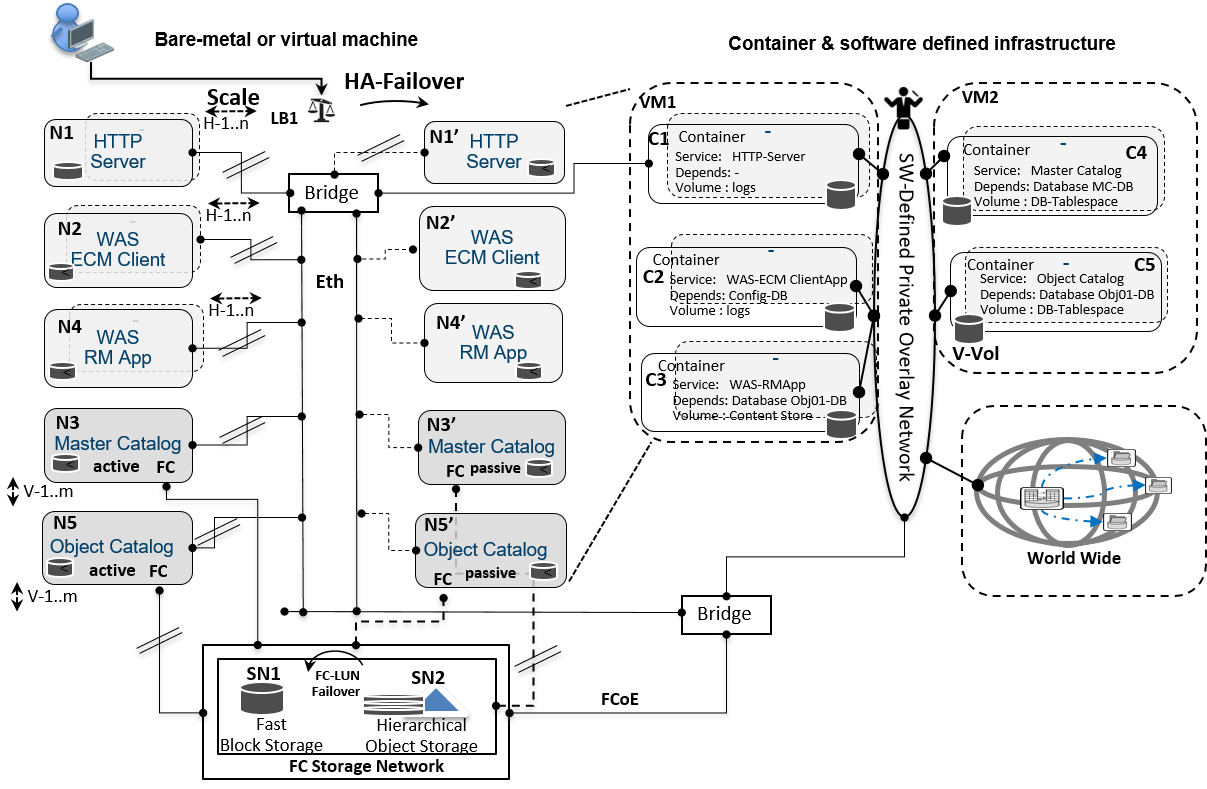
\includegraphics[width=1.0\textwidth]{pics/ECMPic17c.png}
	\caption{Comparison legacy vs cloud physical deployment models of ECM systems}
	\label{fig:ecm-model-implementaion}
	\end{centering}
\end{figure}

    \noindent To mimic a legacy system our implementation of nodes N1-N5 used dedicated virtual machines (VM). Each VM running one of the core components, thus each node in the logical deployment model of Figure~\ref{fig:ecm-model-deployment} is mapped one to one to a virtual machine in Figure~\ref{fig:ecm-model-implementaion}. Every VM is physically connected  to the network and a storage device. Scale for node N1-N3 is achieved by cloning the node (horizontal scale (H-1..n)), instead node N3-N5 (the database nodes) scale vertically (V-1..m). This means system scale and availability (HA,DR) further explodes the deployment topology,shown in Figure ~\ref{fig:ecm-model-deployment} as the right hand side node cluster N1'-N5'. This fact is true for VMs as well as for containers, but the biggest difference is the effort and flexibility to clone a bare-metal or VM production environment compared to expanding and shrinking a containers based environment compared.\\ 
    
    %Legacy systems, due to performance reasons, would normally be configured to run the database nodes N3 and N5 typically on dedicated machines as database administrators hesitated and mistrusted running a RDBMS system on a virtual machine for production. Due to better and more powerful hardware, today, virtual machines have become accepted for running RDBMS in most of the cases. In any case, for our investigation, virtual machines were just fine. Database high availability, due to the transaction oriented nature of database operations, is typically realized by linking two database nodes in a active-passive HA-cluster sharing a dedicated storage and network infrastructure. In this DB-HA configuration, the active node would run in read/write and the passive node in stand-by read-only mode.An aspect that we have emphasized in Fig.~\ref{fig:ecm-model-implementaion} with the labels 'active' and 'passive' on the respective nodes [(N3-N5),(N3'-N5')]. %In Fig.~\ref{fig:ecm-model-implementaion}, we also outline that nodes (N1-N1') representing a high available HTTP-Server pair would be put in a demilitarized zone (DMZ) if required for a secured production system. In the cloud-enabled version, on the right hand side in Figure~\ref{fig:ecm-model-implementaion}, 
    By looking at Figure~\ref{fig:ecm-model-implementaion} you can see that we tried to keep the cloud-enabled version on the right side somewhat symmetrical to reference system on the left in trying to create equivalent systems with respect to functions, scale and availability. The outcome was a fully virtualized and containerized deployment stack capable that supports an automated and faster deployment. First tests also have shown the potential of an elastic provisioning and de-provisioning process based on dynamic load balancing triggers which we are going to evaluate. 
    %\paragraph{Notice} By \textit{virtualized} we mean not just virtual machines but also virtualized storage and network as the overall goal is to fully exploit the capabilities of a software defined production environment. Allowing to spawn containers \textbf{C001-C05} dynamically and to run anywhere in the world of clouds as long as there is a cloud environment to run on and a overlay network to communicate. A fact that we have captured in lower right corner of Figure~\ref{fig:ecm-model-implementaion} 
% -----------------------------------------------------------------------------    
\section{ECM systems design analysis, results and lesson learned}
\label{analysis_and_results}
 The \textbf{short summary} is that our investigation has surfaced several shortcomings and gaps both at design and implementation level preventing an out-of-the-box roll-out into the cloud. Despite this fact, we have found ways and remedies for building a fully virtualized and containerized system based solely on Docker technology that can be used for automating the setup and deployment of an ECM production system in cloud environments. 
 
 %\paragraph{\textbf{Analysis, results}}
    \begin{enumerate}
        \item \textbf{Installation} One of the biggest impediment is that all software products used come optimized for a manual, graphical end-user installation, configuration and setup process. This is a relic from the ancient times installation routines were designed to aid the casual department administrator. Today, that audience is much better served by using ready-to-go docker images container initialization scripts. Current product installation software requires operating systems components just for the installation/configuration process, resulting in a heavier and unnecessary dead code or time consuming work around. \\\\
        \textbf{Lesson learned:} is that the 'Cloud' mandates a paradigm shift, enforced by an automated continuous integration,continuous delivery CI/CD process, thus, making the old GUI-based approach obsolete and allowing to focus more on a flexible scripting interface that eases the task to automate the roll-out of a complete system stack using pre-configure images.
        \item From a \textbf{setup-up and configuration} stand-point, we realized that in the past application and \textit{operational} logic has been mangled and configured in different system components. In the cloud the operational logic must be refactored to use equivalent external cloud services instead. As an example we saw hard coded system topology information and logic at HTTP-Server and Web-Application level designated to handle the distribution of IP-requests among the cluster members and load-balancing is triggered from the inside not from the out-side which becomes counter-productive in highly dynamic cloud environment. \\\\
        \textbf{Lesson learned:}Today's cloud environments provide operational services that make homegrown operational logic obsolete. With refactoring obsolete logic and adding appropriate enhancements legacy systems can be overhauled to consume and exploit cloud services. 
        \item{}Similarly, at storage level in the past resource managers had to monitor and manage pre-assigned storage resources them selves and react to storage shortage or outages, today highly sophisticated storage subsystems are able to provision and de-provision storage on-demand that is highly available and resilient to outages.  \\\\
        \textbf{Lesson learned:} The biggest potential that comes with the cloud is exploiting its elasticity. This means, applications just have to raise a request and the resource is provisioned by cloud services transparently. 
        \item \textbf{System integration test (SIT) and roll-out (PROD)}. Even in our environment bringing up and tear down a test environment with virtual machines took time and lots of efforts. Instead, once we had created the required container images and uploaded them in the docker container image registry, setting up the container based SIT-environment was reduced in running a script, the after test cleaning is just a command. \\\\ 
        \textbf{Lesson learned:} Using the cloud-version all operational jobs (provisioning, de-provisioning, setup, tear-down, scale, fail-over) can be off-loaded to the cloud and best of all it can be done pro-actively at the finest possible service granularity level. Individual application container are spawn dynamically on-demand to run anywhere in the world of clouds as long as there is a system to run on and an overlay network to communicate.
\end{enumerate}  
%-----------------------------------------------------------
\section{Summary and outlook}
\label{conclusions}
    This paper is the result of our research work around the topic on how to re-engineer the architecture design of legacy enterprise content management systems for being able to exploit cloud technologies. The legacy ECM architecture design employs a client-server computing model, and design analysis surfaced a number of design shortcomings and gaps because of the paradigm change that happened during transition from client-server to a cloud-computing model. Our observation is that valid design patterns in the one context become anti-pattern in the other. These facts prevents legacy systems to run properly on cloud environments. The key takeaways are that the legacy of ECM solutions is a somewhat monolithic design, some system components come overloaded with unnecessary operational logic related to pre-configured and hard coded topology knowledge that prevents dynamic on-demand topology changes of a deployed system. To make things worse, product installation and configuration procedures are optimized for a graphical clerical human interface and less for efficient scripting in support of an automated system setup. 

\begin{itemize}
    \item We found several legacy components overloaded with operational logic that shines through several layers, thus, preventing a divide and conquer approach. Here we see the necessity for refactoring these components with a focus on just the business logic. The aim is decompose the application logic in to pieces as small as possible such to fit into self-sufficient containers running in a state-less fashion.
    \item It is important to prevent resource provisioning, deployment topology orchestration as well as workload load-balancing at application level. These functions have to be delegate to the cloud orchestration services by means of application specific deployment templates.  
    \item The use of hardware appliances should be avoided in favor of software defined virtual components. Software Defined Resources like network, storage, load-balancer are part of the cloud platform services. An automated transparent transfer of system topology nodes across a distributed cloud infrastructure is best executed by the cloud orchestrator but request based on business needs and compliance policies. The goal is for the application to declare the \textit{what} is required and leave the \textit{how} it is provisioned to the cloud platform.
    \item Implement system availability (HA,DR) through the use cloud resilience pattern, allowing independent subsystems and services running in their own containers by adopting an architecture style like micro-services.
    \item Make extensive use of the virtualized infrastructure as dedicated or physically attached devices require manual intervention preventing sharing and automation and effectively resulting in lengthy system down times. 
    \item Traditional ECM systems manage the movement of content object through a pre-fined storage hierarchy themselves. Today equivalent services are provided by modern storage system that if used allows to trim down the custom application logic from the respective ECM components.  
\end{itemize}

%-------------------------------------------------------------

%\section{Future Work}
%\label{sect:future-work}
    This work is the first of a trilogy in investigating the best way on how to cloud enable ECM systems. We developed a virtualized and containerized ECM prototype by decomposing the application stack in to smaller components that are confined in stand-alone docker containers and deployed in a virtualized IT-environment. Thus, we outlined a promising approach in to the cloud, where content management can be offered as a service be it on private and hybrid cloud platforms. We showed that through re-engineering it is possible to overcome existing design shortcomings and to close the gaps. Currently we are developing ECM templates for an automated roll-out process based on a Kubernetes Eco-system and are investigating the ability to trigger rule based topology changes proving the feasibility of an elastic topology and  measuring the inertia of the system with respect those changes~\cite{Mega2014}.\\\\
%---------------------------------------------------------
\noindent\textbf{Acknowledgments}
\label{sect:acks}
A big thank you to Gang,Shao that dedicated his master thesis to this work and produced the first containerized version of the cloud prototype~\cite{gang-shao} at the University of Stuttgart.
\label{sect:bib}
\bibliographystyle{plain}
%\bibliographystyle{alpha}
%\bibliographystyle{unsrt}
%\bibliographystyle{abbrv}
\bibliography{ecmforsede2021}

%------------------------------------------------------------
%\appendix{Appendix}
%\begin{enumerate}
%\item
%... Running heads.
%\end{enumerate}
%-----------------------------------------------------------
% Index
%\printindex
%------------------------------------------------------------
\end{document}